\title{Design, Pipelining and Evaluation of a\\Parameterised SIMD Vector Processing Unit on FPGA}

\author{Mahir Abdullah, Krishiv Gupta, Abhiman Singh, Gogulamudi Jayadeep, and Ashish Kushwaha%
\thanks{This paper combines Phase~I and Phase~II of Project 11, SIMD Vector Processing Unit, November 2026.
The authors are with Newton School of Technology, Rishihood University.}%
\thanks{Code, data and all reported results are available at
\url{https://github.com/mahir-m01/SIMD-Vector-Processing-Unit}.}}

\markboth{Design, Pipelining and Evaluation of a Parameterised SIMD Vector Processing Unit on FPGA}%
{Design, Pipelining and Evaluation of a Parameterised SIMD Vector Processing Unit on FPGA}

\maketitle

% =============================================================================
\begin{abstract}
Signal processing, graphics and machine learning apply the same arithmetic to long
arrays of numbers. We present a SIMD vector processing unit in Verilog whose lane
count is a parameter, in two forms that share one 55-instruction set: a
single-cycle core and a four-stage pipelined core. With one lane the same RTL is a
scalar processor, which gives a like-for-like baseline. At eight lanes the unit
holds eight 128-bit vector registers, replicates a 16-operation lane ALU, adds the
lanes in a tree so that a dot-product step is one instruction, and offers
merge-masked execution and saturating arithmetic. Timing analysis of the
single-cycle core showed its critical path in three nearly equal parts, which led to
the pipeline: forwarding, write-through register files, three one-cycle stall rules
and static backward-taken branch prediction. An instruction-level golden model
predicts the exact cycle count of both cores. Every workload, directed test,
mid-run reset and each of 8,000 random programs matches it at 1, 2, 4 and 8 lanes,
and all 23 deliberately planted pipeline bugs are caught. On a Lattice ECP5-25F the
eight-lane single-cycle core reaches 27.1~MHz in 6,135 logic cells and the pipelined
core 50.6~MHz in 8,541. Over eight workloads of 256 elements, eight lanes need
$7.89\x$ (single-cycle) and $7.83\x$ (pipelined) fewer clock cycles than one. In real
time the eight-lane single-cycle core is $5.73\x$ and the eight-lane pipelined core
$10.88\x$ faster than the scalar single-cycle design, and the pipelined core is
$1.90\x$ faster than the single-cycle core at the same lane count. Unrolled loops
raise the figure to $18.6\x$. A problem-size sweep reproduces Amdahl's law.
\end{abstract}

\begin{IEEEkeywords}
Data-level parallelism, data hazards, FPGA, forwarding, golden model, masked
execution, pipelining, saturating arithmetic, SIMD, vector processor, Verilog.
\end{IEEEkeywords}

% =============================================================================
\section{Introduction}\label{sec:intro}

\IEEEPARstart{A}{} scalar processor spends most of its effort on control: fetching,
decoding and sequencing each instruction. When a program adds two arrays, that effort
is repeated for every element, although every element needs the same work. A SIMD
processor issues one instruction for a group of elements, so the control cost is paid
once and the arithmetic is replicated across \emph{lanes}. This is
\emph{data-level parallelism}, the form of parallelism behind vector
supercomputers~\cite{cray1}, multimedia instruction-set extensions~\cite{mmx} and
graphics processors~\cite{hp6}.

\textbf{Problem statement.} The project asks for a small SIMD unit that performs
identical arithmetic and logic operations in parallel, built from a vector register
file, parallel ALUs, a vector control unit, lane multiplexers, a result combiner and
an optional scalar interface. Scalar and SIMD versions of the same workload must be
compared, the vector results verified, and cycle counts, throughput, FPGA resources
and maximum clock frequency measured.

\textbf{Parameterised lanes and a fair baseline.} The lane count $L$ is a parameter of
the Verilog design. With $L = 8$ the vector registers are 128 bits wide. With $L = 1$
the same RTL becomes a scalar processor that runs the same programs with the same
instruction set and timing rules. Any measured gain over the one-lane build therefore
comes from data-level parallelism alone, not from a different microarchitecture.

\textbf{Two design points.} The project was carried out in two phases that now form
one study. The first design point is a \emph{single-cycle} core, in which every
instruction except a load finishes in one clock cycle. It is easy to verify and its
cycle count is exact, but its clock slows as lanes are added, because the whole
datapath lies on one path. The second design point is a \emph{pipelined} core that
splits the same datapath into four stages. Both cores implement the same 55-instruction
set, which adds masked execution and saturating arithmetic to the first design's
instruction set, and both are built, verified and measured with the same flow. The
only difference between them is the pipeline, so the comparison is fair.

We answer six questions with measurements:
\begin{enumerate}
\item How close to the ideal $L\x$ does an $L$-lane unit come in clock cycles, on each
      core?
\item What does each extra lane cost in FPGA logic, multipliers and memory?
\item How much does the wider datapath slow the clock, and where exactly does the
      single-cycle core spend its clock period?
\item What pipeline does that suggest, and can it keep the cycle-exact correctness of
      the single-cycle core at every lane count?
\item How much of the clock-speed gain survives as real speed-up once the cycles the
      pipeline loses to hazards are counted?
\item How do problem size and the order of the instructions change the answer?
\end{enumerate}

The contributions are:
\begin{itemize}
\item a synthesizable SIMD unit in Verilog with a lane count parameter and every block
      named in the brief (Section~\ref{sec:design});
\item a 55-instruction ISA with merge-masked execution and saturating arithmetic, an
      assembler, and a golden model that predicts the results and the exact cycle
      count of both cores (Sections~\ref{sec:isa} and~\ref{sec:tools});
\item a measured critical-path decomposition of the single-cycle core, and a
      four-stage pipelined core with forwarding, write-through register files, three
      stall rules and static branch prediction, in which one forwarding path was
      removed because the timing report showed it cost more than it saved
      (Sections~\ref{sec:why} and~\ref{sec:pipe});
\item a layered verification flow with self-checking testbenches, directed tests,
      random programs, mid-run resets and planted-bug (mutation) tests for both cores
      (Section~\ref{sec:verif});
\item a measured comparison of the two cores in logic, clock speed, cycles and real
      time, with problem-size and unrolling studies (Section~\ref{sec:results}).
\end{itemize}

Section~\ref{sec:lit} reviews related work, Section~\ref{sec:design} describes the
design, its tools and its verification, and Section~\ref{sec:results} presents and
discusses the results. Section~\ref{sec:conclusion} concludes. Fig.~\ref{fig:flow}
shows the flow that produces every result.

\begin{figure*}[t]
\centering
% Combined paper (copy of flow.tex): the flow: how every result in the report is produced.
% Top row: correctness and cycle counts. Bottom row: hardware cost and clock.
\begin{tikzpicture}[x=1mm, y=1mm, font=\scriptsize,
    stage/.style={box, minimum width=24mm, minimum height=11mm},
    key/.style={stage, draw=simd, line width=0.9pt}]

% ---- Top row: simulation ------------------------------------------------------
\node[stage] (prog) at (0,0)    {\textbf{Workloads}\\11 workloads, directed\\and random tests};
\node[stage] (asm)  at (30,0)   {\textbf{Assembler}\\\texttt{vasm.py}\\machine code};
\node[stage] (gold) at (60,8)   {\textbf{Golden model}\\\texttt{golden.py}: memory,\\registers, cycles};
\node[key]   (rtl)  at (60,-8)  {\textbf{RTL simulation}\\both cores, Icarus\\$L = 1, 2, 4, 8$};
\node[key]   (cmp)  at (90,0)   {\textbf{Exact compare}\\all memory words,\\registers, cycles};
\node[stage] (cyc)  at (120,0)  {\textbf{Cycle counts}\\speed-up,\\elements per cycle};

% ---- Bottom row: hardware ----------------------------------------------------------
\node[stage] (mods) at (0,-34)  {\textbf{RTL blocks}\\Verilog modules,\\unit testbenches};
\node[stage] (top)  at (30,-34) {\textbf{FPGA top}\\block RAM, power-on\\reset, LEDs};
\node[stage] (brd)  at (60,-34) {\textbf{Board check}\\registers and memory\\match the model};
\node[key]   (pnr)  at (90,-34) {\textbf{Synthesis, P\&R}\\Yosys + nextpnr,\\ECP5, 3 seeds};
\node[stage] (res)  at (120,-34){\textbf{Resources, $F_{\max}$}\\cells, multipliers,\\block RAM};

% ---- Where the two rows meet -------------------------------------------------------
\node[key] (wall) at (150,-17)  {\textbf{Wall-clock}\\\textbf{speed-up}\\cycles $\times$ clock};

\draw[arr] (prog) -- (asm);
\draw[arr] (asm.east) -- ++(3,0) |- (gold.west);
\draw[arr] (asm.east) -- ++(3,0) |- (rtl.west);
\draw[arr] (gold.east) -- ++(3,0) |- (cmp.west);
\draw[arr] (rtl.east) -- ++(3,0) |- (cmp.west);
\draw[arr] (cmp) -- (cyc);
\draw[arr] (cyc.east) -- ++(4,0) |- (wall.west);
\draw[arr] (res.east) -- ++(4,0) |- (wall.west);

\draw[arr] (mods) -- (top);
\draw[arr] (top) -- (brd);
\draw[arr] (brd) -- (pnr);
\draw[arr] (pnr) -- (res);
\draw[arr] (mods.north) -- (0,-21) -- node[note, above, pos=0.55] {same RTL} (60,-21) -- (rtl.south);
\end{tikzpicture}

\caption{Flow used for every result. Top: each program is assembled once and run on the
golden model and on the RTL of each core at every lane count; memory, registers,
instruction count and cycle count must match exactly. Bottom: the same RTL is wrapped
with block-RAM memories, checked from power-on in simulation, then placed and routed for
resources and maximum clock frequency. Cycle counts and clock frequency together give
the real-time speed-up.}
\label{fig:flow}
\end{figure*}

% =============================================================================
\section{Literature Review}\label{sec:lit}

\subsection{SIMD and Vector Architectures}
Flynn's taxonomy~\cite{flynn72} classifies machines by the number of instruction and
data streams; SIMD names one instruction stream acting on many data elements. The first
commercially successful SIMD designs were vector supercomputers such as the
Cray-1~\cite{cray1}, whose vector registers and pipelined functional units let one
instruction process up to 64 elements, hiding memory latency and avoiding the issue cost
of a scalar loop. Espasa~\emph{et al.}~\cite{espasa98} review the history of vector
architectures and argue that their strengths, few instructions per unit of work and
simple control, suit multimedia workloads. Hennessy and Patterson~\cite{hp6} trace the
same principles from vector machines to subword SIMD and GPUs.

Intel MMX~\cite{mmx} introduced \emph{packed} data types in a general-purpose
processor: one 64-bit register treated as eight bytes or four 16-bit words, with one
instruction operating on all of them. Streaming SIMD Extensions (SSE)~\cite{sse}
widened the registers to 128 bits, the width also used by Arm Neon. Two conventions
from this line of work are adopted here: compare instructions that write all-ones or
all-zeros masks, so that conditionals need no branch, and a fixed 128-bit register
divided into lanes.

VIRAM~\cite{viram} showed that a vector architecture with lanes scales across embedded
media workloads more simply than superscalar or VLIW designs, and that a compiler can
vectorise most kernels automatically. Asanovi\'c~\cite{asanovic98} analysed lane-based
vector microprocessors in depth, and Lee~\emph{et al.}~\cite{maven} found vector cores
more efficient than MIMD, subword-SIMD and SIMT designs even on fairly irregular
kernels. Two current ISAs leave the vector length to the implementation: the RISC-V
vector extension~\cite{rvv} and the Arm Scalable Vector Extension, which allows
registers from 128 to 2048 bits under one vector-length-agnostic programming
model~\cite{sve}. Ara~\cite{ara} implements RISC-V V with identical lanes, each holding
a slice of the vector register file, and reaches over 1~GHz in 22-nm technology. The
lane replication used in this project follows the same idea at a much smaller scale.

Table~\ref{tab:isas} compares this unit with instruction sets in use today. Intel SSE2
and AVX2~\cite{intelsdm}, Arm Neon~\cite{armarm} and the MIPS SIMD Architecture
(MSA)~\cite{msa} fix the register width in the ISA; RISC-V V lets one binary run on any
width through \texttt{vsetvli}. Three conventions are adopted here. The 128-bit
register and the all-ones compare mask follow SSE, Neon and MSA. The vector--scalar form
follows RISC-V V's \texttt{.vx} instructions, which broadcast a scalar register inside
the instruction. A full sum across lanes follows Neon's \texttt{ADDV} and RISC-V V's
\texttt{vredsum}, whereas x86 \texttt{PMADDWD} and MSA \texttt{DOTP\_S} only add
products in pairs; those two keep each product at 32 bits, while \texttt{VDOT} keeps its
low 16 bits.

\begin{table}[t]
\centering
\caption{SIMD Instruction Sets Compared}
\label{tab:isas}
\scriptsize
\setlength{\tabcolsep}{2.6pt}
\begin{tabular}{llllll}
\toprule
ISA & Width (bits) & Regs & Int.\ el. & Sum across lanes & Conditionals \\
\midrule
SSE2       & 128           & 8/16 & 8--64 & pairs (\texttt{PMADDWD})  & mask, blend \\
AVX2       & 256           & 16   & 8--64 & pairs (\texttt{VPMADDWD}) & mask, blend \\
Neon (A64) & 128           & 32   & 8--64 & full (\texttt{ADDV})      & mask, \texttt{BSL} \\
MIPS MSA   & 128           & 32   & 8--64 & pairs (\texttt{DOTP\_S})  & mask \\
RISC-V V   & \texttt{VLEN} & 32   & 8--64 & full (\texttt{vredsum})   & mask in \texttt{v0} \\
This work  & $16L$ (128)   & 8    & 16    & full, 16-bit products     & mask, mask reg.\ \\
\bottomrule
\end{tabular}
\end{table}

\subsection{Soft Vector Processors on FPGAs}
FPGAs suit lane-replicated designs because the lane count can be matched to the device.
VESPA~\cite{vespa} showed a soft vector processor whose lane count and width can be
scaled and customised to each application. VIPERS~\cite{vipers} used a soft vector unit
as a general-purpose accelerator for a Nios~II processor and reported up to $44\x$
speed-up over a Nios~II/s with 32 lanes, at $26\x$ its area. VEGAS~\cite{vegas}
replaced the vector register file with a scratchpad and introduced fracturable ALUs,
and the VectorBlox MXP~\cite{mxp} turned these ideas into a commercial core with 1 to
over 128 ALUs. Vicuna~\cite{vicuna} is an open-source RISC-V vector coprocessor designed
so that its execution time is predictable, which allows tight worst-case timing
analysis. These designs map lane-replicated, pipelined datapaths onto FPGA DSP blocks
and block RAM. Most of them report speed-up against a separate host processor, so the
baseline differs from the vector unit in microarchitecture as well as in width. Our
unit is far smaller, but it meets the same structures in its timing: the block-RAM
access time and the cross-lane adder tree dominate its single-cycle path
(Section~\ref{sec:why}).

\subsection{Pipelining, Hazards and Branch Prediction}
Pipelining overlaps the execution of successive instructions in stages separated by
registers, so that the clock period covers one stage instead of the whole
instruction~\cite{hp6, pattersonrv}. The cost is hazards. A data hazard arises when an
instruction needs a result that an older instruction has not yet written. The classic
five-stage RISC pipeline resolves most of them by forwarding results from later stages
to the inputs of the execute stage, and stalls for one cycle when a load's data is used
by the very next instruction, because that data arrives too late to
forward~\cite{pattersonrv}. Writing the register file in the first half of the cycle
and reading it in the second half removes the hazard between instructions two apart; a
write-through (bypassing) register file achieves the same with a multiplexer per read
port. A control hazard arises because the next instruction must be fetched before a
branch is resolved. Static prediction guesses without history; among the strategies
Smith compared is to predict backward branches taken and forward branches not taken
(BTFN)~\cite{smith81}, which suits loops, whose closing branch is backward and almost
always taken, and needs only the sign of the offset. Dynamic predictors do better on
irregular code but need tables, which a small loop-dominated accelerator does not
justify.

\subsection{Predication, Masking and Saturation}
Conditional code in data-parallel loops cannot branch per lane. If-conversion turns
control dependence into data dependence: both outcomes are computed and a predicate
selects between them~\cite{allen83}. Packed SIMD extensions such as SSE and Neon do
this with compare results used as bit masks and explicit blend or select
instructions~\cite{sse, armarm}. Vector architectures instead predicate the
instruction itself: the Cray-1 had a vector mask register~\cite{cray1}, RISC-V V masks
any instruction with register \texttt{v0}~\cite{rvv}, Arm SVE has sixteen predicate
registers~\cite{sve} and AVX-512 eight opmask registers~\cite{intelsdm}. Two policies
exist for the inactive lanes: merging keeps their old destination value, zeroing clears
them. Merging needs the old value, which in hardware means either an extra
register-file read port or per-lane write enables.

Media instruction sets added saturating addition because wrap-around is the worst
possible answer for pixels and audio samples: a bright pixel that overflows becomes
black~\cite{mmx}. Signed saturating addition is now standard in SSE2, Neon, MSA and
RISC-V V~\cite{intelsdm, armarm, msa, rvv}.

\subsection{Scheduling, Problem Size and Performance Limits}
Stalls in an in-order pipeline can be removed in software by placing independent
instructions between a producer and its consumer; loop unrolling both creates such
independent instructions and amortises the loop overhead~\cite{dongarra79, hp6}.
Amdahl's law~\cite{amdahl} bounds the speed-up of any parallel unit by the fraction of
work that stays serial; in a vector loop that fraction is the set-up code, the loop
control and the final reduction. Gustafson's observation~\cite{gustafson} that larger
problems shrink the serial fraction explains why speed-up grows with array length.

\subsection{Verification and Tools}
Comparing a design against an independent instruction-level model is standard practice
in processor verification, and mutation testing~\cite{demillo} judges a test suite by
whether it detects deliberately injected faults. Open-source flows make resource and
timing results reproducible: Icarus Verilog~\cite{icarus} simulates,
Verilator~\cite{verilator} lints, and Yosys~\cite{yosys} with nextpnr~\cite{nextpnr}
synthesise, place and route designs for the Lattice ECP5 using documented timing models.

\subsection{Gap Addressed}
Published soft vector processors are large and are usually compared against a different
scalar core. This project builds a design small enough for every line to be explained
and verified. Its scalar baseline is the \emph{same} RTL with one lane, and its two cores
differ only in the pipeline, so measured gains can be attributed to data-level
parallelism and to pipelining separately. Its timing is as predictable as Vicuna's in a
far simpler form: the cycle count of every program follows from its instruction, load,
stall and branch counts.

% =============================================================================
\section{Proposed Solution}\label{sec:design}

\subsection{Design Goals and Parameters}
The first goal is clarity and exactness: every block is small, and the cycle count of a
program is predictable from simple rules. The second is speed on the FPGA, which the
pipelined core adds without changing the instruction set. Two parameters set the shape
(Table~\ref{tab:params}): the number of lanes $L$ and the element width $W = 16$ bits.
With $L = 8$ a vector holds $8 \times 16 = 128$ bits, the width of SSE and Neon
(Fig.~\ref{fig:lanes}). The memories sit outside the core, so the same RTL is used in
simulation and on the FPGA. The RTL is plain Verilog (IEEE
1364-2005~\cite{ieee1364}): one module per block, \texttt{generate} loops for the lanes
and no vendor primitives. A decoder module is shared by both cores, so they cannot
disagree about what an instruction means.

\begin{table}[t]
\centering
\caption{Design Parameters}
\label{tab:params}
\footnotesize
\begin{tabular}{llL{0.48\columnwidth}}
\toprule
Parameter & Value & Meaning \\
\midrule
\texttt{LANES} ($L$) & 1, 2, 4, 8 & lanes in parallel (default 8) \\
\texttt{W}           & 16         & bits per element (signed) \\
vector registers     & $8 \times 16L$ bits & \texttt{v0}--\texttt{v7} \\
lane mask            & $L$ bits   & one bit per lane, all on at power-up \\
scalar registers     & $8 \times 32$ bits  & \texttt{s0}--\texttt{s7}, \texttt{s0} always 0 \\
\texttt{IADDR\_W}    & 8          & 256 instructions \\
\texttt{DADDR\_W}    & 10         & 1,024 data words (also on the FPGA) \\
\texttt{BYPASS}      & 0, 1       & register-file write-through (1 in the pipelined core) \\
\bottomrule
\end{tabular}
\end{table}

\begin{figure}[t]
\centering
\input{figures/lanes.tex}
\caption{One SIMD instruction. A 128-bit register holds eight 16-bit elements, one per
lane, and \texttt{VADD} adds all eight pairs at once. Lanes are independent: no carry
crosses a lane boundary (dashed). The scalar build ($L = 1$) runs the same program with
one element per register.}
\label{fig:lanes}
\end{figure}

\subsection{Instruction Set}\label{sec:isa}
Instructions are 32 bits: a 6-bit opcode, three 3-bit register fields, a mask flag in
bit~16 and a signed 16-bit immediate (Fig.~\ref{fig:format}). The two top opcode bits
select one of four classes (Table~\ref{tab:isa}); in the first three, the low four bits
select one of 16 ALU jobs: \texttt{ADD}, \texttt{SUB}, \texttt{AND}, \texttt{OR},
\texttt{XOR}, three shifts (\texttt{SLL}, \texttt{SRL}, \texttt{SRA}, by $b \bmod 16$),
\texttt{MUL} (low 16 bits), \texttt{SEQ}, \texttt{SLT}, \texttt{SLTU}, \texttt{MIN},
\texttt{MAX} and the saturating \texttt{ADDS} and \texttt{SUBS}. Sixteen jobs in three
forms plus seven memory, mask, scalar and control instructions give 55 instructions;
the first design had 14 jobs and 48 instructions, and the two saturating jobs and
\texttt{VMSK} are the additions, together with the use of bit~16. Compare jobs write
\texttt{0xFFFF} for true and 0 for false, so a result can be used directly as a mask with
\texttt{VAND}. Arithmetic wraps around on overflow ($32767 + 1 = -32768$) except in the
saturating jobs ($32767 + 1 = 32767$). Data addresses wrap modulo the memory size and the
program counter wraps after 255. Unused opcodes in class \texttt{11} do nothing for one
cycle, so every bit pattern has a defined effect.

\begin{figure}[t]
\centering
% Combined paper: the 32-bit instruction word with the mask bit and 16 jobs (copy of format.tex).
% One bit = 1.8 mm. Field values under each box are binary (imm in hex).
\begin{tikzpicture}[x=1mm, y=1mm, font=\scriptsize,
    field/.style={draw=edge, minimum height=6mm, inner sep=0pt, line width=0.5pt, anchor=south west},
    bits/.style={font=\tiny, text=edge},
    val/.style={font=\tiny\ttfamily}]

% Field boxes: (left edge, width, label, fill)
\foreach \x/\w/\t/\f in {0/10.8/opcode/simdfill, 10.8/5.4/rd/white, 16.2/5.4/ra/white,
                         21.6/5.4/rb/white, 27/1.8/m/simdfill, 28.8/28.8/{imm (signed)}/white}
  \node[field, minimum width=\w mm, fill=\f] at (\x,0) {\t};

% Bit numbers: the top bit of each field, and bit 0.
\foreach \x/\b in {0.9/31, 11.7/25, 17.1/22, 22.5/19, 29.7/15, 56.7/0}
  \node[bits] at (\x, 7.8) {\b};

% Four encodings (mnemonic on the left, field values under each box).
\foreach \y/\m/\op/\rd/\ra/\rb/\imm/\hex in {
    -4/{VADD v3, v1, v2}/000000/011/001/010/0000/01940000,
    -8/{VMUL v1, v1, s3}/011000/001/001/011/0000/60960000,
   -12/{VDOT s4, v1, v2}/101000/100/001/010/0000/A2140000,
   -16/{VLD v1, 4(s1)}/110000/001/001/000/0004/C0900004} {
  \node[val, anchor=east] at (-0.6, \y) {\m};
  \node[val] at (5.4, \y) {\op};  \node[val] at (13.5, \y) {\rd};
  \node[val] at (18.9, \y) {\ra}; \node[val] at (24.3, \y) {\rb};
  \node[val] at (27.9, \y) {0};   \node[val] at (43.2, \y) {0x\imm};
  \node[val, text=edge, anchor=west] at (58.6, \y) {\hex};
}

% Opcode split: class in the top two bits, ALU job in the low four.
\draw[decorate, decoration={brace, amplitude=2pt, mirror}, edge] (0, -18.5) -- (10.8, -18.5);
\node[note, align=left, anchor=north west, text width=78mm, inner sep=0pt] at (-14, -21)
  {\textbf{opcode} = class (2 bits) + job (4 bits).
   Class \texttt{00} vector--vector, \texttt{01} vector--scalar, \texttt{10} reduce,
   \texttt{11} memory and control. The job picks one of the 16 ALU operations; bit 16 (m) marks a masked instruction.};
\end{tikzpicture}

\caption{Instruction format and four encodings produced by the assembler (right: the
32-bit word in hexadecimal). Bit 16 (m) is the mask flag and is 0 in all four.}
\label{fig:format}
\end{figure}

\begin{table}[t]
\centering
\caption{Instruction Classes ($i$ Runs Over All Lanes)}
\label{tab:isa}
\footnotesize
\setlength{\tabcolsep}{3.5pt}
\begin{tabular}{lll}
\toprule
Instruction & Opcode & Effect \\
\midrule
\texttt{V}\emph{op} \texttt{vd, va, vb} & \texttt{0x00}--\texttt{0x0F} & $v_d[i] = v_a[i] \circ v_b[i]$ \\
\texttt{V}\emph{op} \texttt{vd, va, sb} & \texttt{0x10}--\texttt{0x1F} & $v_d[i] = v_a[i] \circ s_b$ (broadcast) \\
\texttt{VRED}\emph{op} \texttt{sd, va, vb} & \texttt{0x20}--\texttt{0x2F} & $s_d = \sum_i \left(v_a[i] \circ v_b[i]\right)$ \\
\texttt{VLD vd, imm(sa)}  & \texttt{0x30} & $v_d = M[s_a + \mathit{imm}]$ \\
\texttt{VST vb, imm(sa)}  & \texttt{0x31} & $M[s_a + \mathit{imm}] = v_b$ \\
\texttt{VMSK va}          & \texttt{0x34} & mask$[i] = [v_a[i] \neq 0]$ \\
\texttt{ADDI sd, sa, imm} & \texttt{0x38} & $s_d = s_a + \mathit{imm}$ \\
\texttt{ADD sd, sa, sb}   & \texttt{0x39} & $s_d = s_a + s_b$ \\
\texttt{BNE sa, sb, label}& \texttt{0x3C} & branch if $s_a \neq s_b$ \\
\texttt{HALT}             & \texttt{0x3F} & stop \\
\bottomrule
\end{tabular}
\end{table}

\texttt{VDOT} is another name for \texttt{VREDMUL}: a dot-product step in one
instruction. As with \texttt{VMUL}, each product keeps its low 16 bits before the
32-bit sum. The vector-add kernel shows the style of every workload:
\begin{lstlisting}
      ADDI s1, s0, 0       # word index
      ADDI s2, s0, ITER    # passes = N / L
loop: VLD  v1, A(s1)
      VLD  v2, B(s1)
      VADD v3, v1, v2      # L additions at once
      VST  v3, C(s1)
      ADDI s1, s1, 1
      BNE  s1, s2, loop
      HALT
\end{lstlisting}
The same source runs on every lane count; only the constant \texttt{ITER} changes.

\subsection{Microarchitecture}\label{sec:micro}
Fig.~\ref{fig:block} shows the single-cycle core with eight lanes. Following one
instruction, \texttt{VMUL v3, v1, s2}, through it: the control unit decodes class
\texttt{01} and job \texttt{MUL}; the vector register file reads \texttt{v1} while the
scalar register file reads \texttt{s2}; the lane multiplexers copy the low 16 bits of
\texttt{s2} into every lane; all eight ALUs multiply at once; and at the next clock edge
the combined 128-bit result is written to \texttt{v3}. In the single-cycle core all of
this happens within one clock cycle. The pipelined core uses the same blocks, spread over
four cycles (Section~\ref{sec:pipe}).

\begin{figure*}[t]
\centering
\input{figures/block.tex}
\caption{Block diagram of the single-cycle core with eight lanes. Blue: vector
datapath; orange: scalar side; grey: control and memories; dashed: control signals. The
instruction and data memories are synchronous block RAM outside the core. The lane mask
and the register-file write-through paths are not drawn.}
\label{fig:block}
\end{figure*}

\textbf{Vector control unit.} Decodes each instruction into control signals and
computes the next program counter. Instruction memory is synchronous, so in the
single-cycle core the unit sends it the address of the \emph{next} instruction one cycle
early, including the target of a taken branch; branches therefore cost no extra cycle.
A load takes two cycles: the address goes out in the first while the program counter
holds, and the returned data is written in the second.

\textbf{Vector register file.} Eight $16L$-bit registers with two asynchronous read
ports and one synchronous write port. Each lane has its own write enable, so a masked
write changes only the active lanes and the old value is never read back, which needs
no third read port. One extra register, the lane mask, holds one bit per lane. With the
\texttt{BYPASS} parameter set the file is \emph{write-through}: a read of the register
being written in the same cycle returns the new value, lane by lane. The single-cycle
core uses \texttt{BYPASS} = 0, because there the reading instruction is the one
writing, and a write-through would feed the result back into its own inputs; the
pipelined core uses \texttt{BYPASS} = 1.

\textbf{Scalar register file (scalar interface).} Eight 32-bit registers, with
\texttt{s0} hard-wired to zero and the same two modes. They hold addresses, loop
counters, broadcast values and reduction results. A third, debug read port exposes any
register to the testbench, or to the LEDs on the board.

\textbf{Lane multiplexers.} For each lane, operand B is either that lane's element of
$v_b$ or the low 16 bits of $s_b$ copied into every lane. Without the broadcast,
multiplying a vector by a constant would need a vector full of copies of it.

\textbf{Parallel ALUs.} $L$ copies of a combinational 16-operation lane ALU, created
with a \texttt{generate} loop and sharing one operation code. Lanes have no connection
to each other. The saturating jobs compute the sum with one extra bit, so it cannot
overflow; when the top two bits of the 17-bit result differ, the true value lies outside
$[-32768, 32767]$ and the top bit selects the limit. On the ECP5 each lane's multiply
uses one hardware multiplier block.

\textbf{Result combiner.} Passes the lane outputs on as one vector for write-back. For
reduce instructions it also sign-extends them to 32 bits and adds them in a
$\log_2 L$-level adder tree (Fig.~\ref{fig:combiner}), so the sum cannot overflow. For
masked reductions a lane that is switched off enters the tree as 0, one AND gate per
input bit in front of the first level. The combiner also outputs one flag per lane that
is 1 when the lane's result is non-zero, which \texttt{VMSK} stores as the new mask.

\textbf{FPGA top.} Adds block-RAM instruction and data memories loaded at power-up, a
power-on reset that holds the core for 15 clocks, a two-flip-flop synchroniser on the
reset button, three switches that select a scalar register and eight LEDs that show its
low byte. It builds either core.

\begin{figure}[t]
\centering
\input{figures/combiner.tex}
\caption{Result combiner for eight lanes. Reduce instructions widen each lane result to
32 bits and sum them in $\log_2 8 = 3$ levels of adders; vector instructions use the
lane results directly as the destination vector.}
\label{fig:combiner}
\end{figure}

\subsection{Masked Execution and Saturating Arithmetic}\label{sec:mask}
Bit~16 marks a vector or reduce instruction as masked (suffix \texttt{.M} in the
assembler). A masked vector instruction \emph{merges}: lanes whose mask bit is 0 keep the
old value of $v_d$. A masked reduction adds only the active lanes. \texttt{VMSK} $v_a$
sets the mask to one bit per lane, $m_i = [v_a[i] \neq 0]$, so a compare followed by
\texttt{VMSK} activates exactly the lanes where the compare was true. It runs on the
existing hardware as $v_a \,|\, s_0$ with $s_0 = 0$, using the result combiner's lane
flags. The mask resets to all ones at power-up. The absolute value of every lane needs no
branch:

\noindent\begin{minipage}{\columnwidth}
\begin{lstlisting}
      VSLT    v2, v1, s0   # ones where v1 < 0
      VMSK    v2           # mask = those lanes
      VSUBS.M v1, v3, v1   # v1 = 0 - v1 (v3 = 0)
\end{lstlisting}
\end{minipage}

The saturating jobs \texttt{ADDS} and \texttt{SUBS} are available in all three forms and
let the \texttt{brighten} workload clamp pixel values at 32767 instead of wrapping to
negative numbers.

\subsection{Single-Cycle Core Timing Model}\label{sec:timing}
Every instruction except \texttt{VLD} completes in one cycle (Fig.~\ref{fig:timing}),
so the run time of a program is
\begin{equation}
  \text{cycles} = \text{instructions} + \text{loads}.
  \label{eq:cycles}
\end{equation}
For a kernel with $k$ set-up instructions, a loop body of $b$ instructions containing
$\ell$ loads, and $N$ elements on $L$ lanes,
\begin{equation}
  C(L) = k + \frac{N}{L}\,(b + \ell) + 1, \qquad
  S(L) = \frac{C(1)}{C(L)} < L,
  \label{eq:model}
\end{equation}
where the final 1 is \texttt{HALT}. The speed-up $S$ approaches $L$ as $N$ grows; the
$k + 1$ serial instructions are the Amdahl term.

\begin{figure}[t]
\centering
\input{figures/timing.tex}
\caption{One pass of the vector-add loop on the single-cycle core at the cycle level.
Each \texttt{VLD} holds the program counter for one cycle and writes its register in the
second. In cycle 7 the taken \texttt{BNE} already sends the loop start (address 2,
orange) to instruction memory, so the branch costs nothing.}
\label{fig:timing}
\end{figure}

\subsection{Where the Single-Cycle Core Spends Its Clock}\label{sec:why}
The first build of the single-cycle core, with the 48-instruction set that lacked masks
and saturation, used 5,396 ECP5 logic cells and reached 29.1~MHz at eight lanes, a
real-time speed-up of $5.3\x$ over its own scalar configuration. With the final
55-instruction set the single-cycle core measures 6,135 cells and 27.1~MHz
(Section~\ref{sec:fpga}); all later numbers refer to the final builds. The cycle count of
the first build was already within 2\% of ideal, so the gap was in the clock: the
frequency fell by a third from one lane to eight.

We read the critical path of that first eight-lane build from nextpnr's timing report
(ECP5-25F, speed grade~6, seed~1). It was 34.7~ns long and fell into three nearly equal
parts: instruction fetch, decode and the LUT-RAM register read, about 12.8~ns together
(5.6~ns of it the block RAM's clock-to-output time); the lane multiplier and its result
multiplexer, about 9~ns; and the three-level adder tree of the reduction with the write
into the scalar register file, about 12.7~ns. Three balanced pieces suggest registers
between them, which gives the four-stage pipeline of Fig.~\ref{fig:pipe}.

\subsection{Pipelined Core}\label{sec:pipe}
\textbf{Stages.} Fetch (F) is the instruction block RAM; decode (D) decodes, reads the
write-through register files, guesses branches and runs the hazard unit; execute (X)
holds the forwarding select, the lane multiplexers and ALUs, the scalar adder, the
data-memory access and the branch check; write (W) adds the lanes for reductions, flags
non-zero lanes for \texttt{VMSK} and selects the value to write
(Fig.~\ref{fig:pipe}). The instruction memory's own output register is the boundary
between fetch and decode, as in the single-cycle core, so the pipeline adds two
registers: D/X, which holds the decoded control signals and the operands read in D, and
X/W, which holds the lane results, the scalar adder's result and the lane enables. The
shared decoder also lists which registers an instruction reads and writes, which the
hazard unit needs. Every pipeline-register field carries a valid bit, and nothing that
changes state (a memory write, a register write, a branch correction) acts on an invalid
entry.

\begin{figure*}[t]
\centering
% Pipelined core: four stages, three pipeline registers, and the paths that
% handle hazards (forwarding, write-through, branch guess and check, stall).
% Blue = vector datapath, orange = scalar side, grey = control and memories.
% Dashed = control.
\begin{tikzpicture}[x=1mm, y=1mm, font=\footnotesize,
    blk/.style={box, minimum height=9mm, inner sep=2pt},
    vblk/.style={blk, fill=simdfill, draw=simd},
    sblk/.style={blk, fill=scalfill, draw=scal},
    gblk/.style={blk, fill=greyfill},
    preg/.style={draw=edge, fill=greyfill, minimum width=2.6mm, minimum height=56mm, inner sep=0pt},
    stage/.style={font=\small\bfseries, text=edge},
    lbl/.style={note}]

% ---- Stage titles and pipeline registers ----------------------------------------
\node[stage] at (9,50)   {F: fetch};
\node[stage] at (50,50)  {D: decode};
\node[stage] at (107,50) {X: execute};
\node[stage] at (157,50) {W: write};

\node[preg] (fd) at (24,4) {};  \node[lbl, above=0.5mm] at (fd.north) {RAM out};
\node[preg] (dx) at (78,4) {};  \node[lbl, above=0.5mm] at (dx.north) {D/X};
\node[preg] (xw) at (136,4) {}; \node[lbl, above=0.5mm] at (xw.north) {X/W};

% ---- F ---------------------------------------------------------------------------
\node[gblk, minimum width=17mm] (imem) at (9,14)  {Instruction\\memory};
\node[gblk, minimum width=17mm] (fsel) at (9,-14) {Next fetch\\address};

% ---- D ---------------------------------------------------------------------------
\node[gblk, minimum width=24mm] (dec)  at (42,24)  {Decoder};
\node[gblk, minimum width=13mm] (guess) at (66,24) {Branch\\guess};
\node[vblk, minimum width=34mm] (vrf)  at (51,9)   {Vector registers + mask\\\scriptsize write-through};
\node[sblk, minimum width=34mm] (srf)  at (51,-4)  {Scalar registers\\\scriptsize write-through};
\node[gblk, minimum width=34mm] (haz)  at (51,-14) {Hazard unit\\\scriptsize stall $\cdot$ forwarding select};

% ---- X ---------------------------------------------------------------------------
\node[vblk, minimum width=7mm, minimum height=26mm, font=\scriptsize] (fwd) at (87,4) {};
\node[font=\scriptsize, rotate=90] at (fwd.center) {forwarding select};
\node[vblk, minimum width=14mm] (mux)  at (102,13) {Lane\\MUX};
\node[vblk, minimum width=16mm] (alus) at (122,13) {8 lane\\ALUs};
\node[sblk, minimum width=14mm] (sadd) at (102,-4) {Scalar\\adder};
\node[gblk, minimum width=16mm] (dmem) at (122,-4) {Data\\memory};
\node[gblk, minimum width=14mm] (bchk) at (102,-17){Branch\\check};

% ---- W ---------------------------------------------------------------------------
\node[vblk, minimum width=26mm] (comb) at (157,13) {Result combiner\\\scriptsize adder tree $\cdot$ lane flags};
\node[gblk, minimum width=26mm] (wsel) at (157,-6) {Result select\\\scriptsize lanes / sum / load};

% ---- Main flow -------------------------------------------------------------------
\draw[arr] (imem.east) -- (fd.west |- imem.east);
\draw[arr] (fd.east |- dec.west) -- (dec.west);
\draw[arr] (dec.south) -- (dec.south |- vrf.north);
\draw[arr] (vrf.east) -- (dx.west |- vrf.east);
\draw[arr] (srf.east) -- (dx.west |- srf.east);
\draw[arr] (dx.east |- 0,13) -- (fwd.west |- 0,13);
\draw[arr] (dx.east |- 0,-4) -- (fwd.west |- 0,-4);
\draw[arr] (fwd.east |- mux.west) -- (mux.west);
\draw[arr] (mux.east) -- (alus.west);
\draw[arr] (fwd.east |- sadd.west) -- (sadd.west);
\draw[arr] (sadd.east) -- node[above, lbl]{addr} (dmem.west);
\draw[arr] (fwd.east |- 0,-7) -- (94,-7) |- (bchk.west);
\draw[arr] (alus.east) -- (xw.west |- alus.east);
\draw[arr] (dmem.east) -- (xw.west |- dmem.east);
\draw[arr] (xw.east |- comb.west) -- (comb.west);
\draw[arr] (xw.east |- wsel.west) -- node[above, lbl, pos=0.45]{load} (wsel.west);
\draw[arr] (comb.south) -- (wsel.north);

% ---- Forwarding: W back to the operands in X ----------------------------------------
\draw[arr, draw=simd, line width=0.8pt] (wsel.east) -- (176,-6) -- (176,38) -- node[above, lbl, pos=0.5]{forwarding: the result in W replaces a stale operand in X} (87,38) -- (fwd.north);

% ---- Write-back into the register files, seen at once in D ----------------------------
\draw[arr, draw=simd, line width=0.8pt] (wsel.south) -- (157,-35) -- node[below, lbl, pos=0.5]{write-back; write-through makes it visible to D in the same cycle} (30,-35) -- (30,9) -- (vrf.west);
\draw[arr, draw=scal, line width=0.8pt] (30,-4) -- (srf.west);

% ---- Branches and stalls --------------------------------------------------------------
\draw[arr, dashed] (dec.east) -- (guess.west);
\draw[arr, dashed] (guess.north) -- (66,41) -- node[above, lbl, pos=0.55]{backward branch: fetch its target next} (2,41) -- (2,-14) -- (fsel.west);
\draw[arr, dashed] (bchk.south) -- (102,-28) -- node[below, lbl, pos=0.45]{wrong guess: drop the instruction in D, fetch the right one} (9,-28) -- (fsel.south);
\draw[arr, dashed] (haz.west) -- node[below, lbl, pos=0.15]{stall} (fsel.east |- haz.west);
\draw[arr] (fsel.north) -- node[right, lbl]{address} (imem.south);
\end{tikzpicture}

\caption{The pipelined core. Fetch (F) is the instruction block RAM; decode (D) reads
the write-through register files, guesses backward branches taken and runs the hazard
unit; execute (X) holds the forwarding select, the lane multiplexers and ALUs, the
scalar adder, the data-memory access and the branch check; write (W) adds the lanes for
reductions, flags non-zero lanes for \texttt{VMSK} and selects the value to write. Blue
lines carry the result back: forwarded from W to X, and written through to D.}
\label{fig:pipe}
\end{figure*}

\textbf{Data hazards.} Three mechanisms keep results correct. (i)~Forwarding: when the
instruction in X reads a register that the instruction in W is writing, it takes the
value from the X/W register instead of the stale copy read in D. (ii)~Write-through
register files: an instruction two places behind a producer reads its registers in D
while the producer writes in W; the register files return the value being written in
the same cycle, lane by lane, so nothing more is needed. (iii)~Stalls: three kinds of
result are not available at the start of W and are not forwarded
(Table~\ref{tab:stalls}). When the instruction in D needs one of them from the
instruction in X, D holds for one cycle and a bubble enters X; a cycle later the
producer is in W and the write-through file supplies the value. A reduction into
\texttt{s0} writes nothing and never causes a stall.

\begin{table}[t]
\centering
\caption{Results That Make the Next Instruction Wait One Cycle}
\label{tab:stalls}
\footnotesize
\begin{tabular}{@{}L{1.7cm}L{3.4cm}L{2.5cm}@{}}
\toprule
Producer & Why it is not forwarded & Example \\
\midrule
reduction & the adder tree sums the lanes during W & \texttt{VDOT s4} then \texttt{ADD s3, s3, s4} \\
masked vector op & inactive lanes must keep the old value, held only by the register file & \texttt{VADD.M v3} then \texttt{VST v3} \\
load & data arrives from block RAM during W; forwarding it into the multiplier slowed the clock (Section~\ref{sec:fwdload}) & \texttt{VLD v2} then \texttt{VADD v3, v1, v2} \\
\bottomrule
\end{tabular}
\end{table}

\textbf{Control hazards.} Branches are checked in X, against forwarded operands. In D,
a branch with a negative offset is guessed taken and its target is fetched at once; a
forward branch is guessed not taken. A wrong guess turns the one wrongly fetched
instruction in D into a bubble and fetches the correct address, so it costs one cycle;
a loop's branch is wrong only at its exit. The guess uses the sign bit of the full
16-bit offset.

\textbf{Halting and reset.} Once \texttt{HALT} leaves D, D stops passing instructions
on; a \texttt{HALT} fetched on a wrong path never leaves D because the wrong guess
removes it first. The \texttt{halted} flag rises when \texttt{HALT} leaves X, at the same
clock edge at which the last older instruction is written in W. Reset invalidates every
stage and blocks every write while it is held.

\textbf{Loads and cycle count.} \texttt{VLD} sends its address in X and writes its data in
W, so a load occupies one cycle instead of the two of the single-cycle core. With these
rules the pipelined core needs
\begin{equation}
C_{\mathrm{pipe}} = I + 1 + S + M
\label{eq:pipe}
\end{equation}
cycles, where $I$ is the number of instructions executed, the 1 fills the pipeline, $S$
counts stalls and $M$ wrong branch guesses. For the loop kernels $M = 1$ and, with
$\sigma$ stalls per pass, \eqref{eq:model} becomes
$C_{\mathrm{pipe}}(L) = k + 3 + (N/L)(b + \sigma)$. The two fixed terms, the pipeline
fill and the wrong guess at the loop exit, do not shrink with $L$. Fig.~\ref{fig:ptiming}
shows one pass of the \texttt{vadd} loop.

\begin{figure*}[t]
\centering
% Pipeline timing of one vadd loop pass on the pipelined core: the
% load-use stall (VADD waits for v2), forwarding (VST gets v3 from W) and the
% backward branch guessed taken (the next pass starts at once).
\begin{tikzpicture}[x=7.4mm, y=5.2mm, font=\scriptsize]
  \tikzset{st/.style={draw=edge, minimum width=6.6mm, minimum height=4.4mm, inner sep=0pt, font=\scriptsize},
           F/.style={st, fill=greyfill}, D/.style={st, fill=simdfill}, X/.style={st, fill=simdfill, draw=simd},
           W/.style={st, fill=white}, B/.style={st, fill=scalfill, draw=scal}}
  % cycle numbers
  \foreach \c in {1,...,10} \node[text=edge] at (\c+1.6, 0.9) {\c};
  \node[text=edge, anchor=east] at (2.0, 0.9) {cycle};
  % instructions (row, label)
  \foreach \r/\t in {0/{VLD v1, A(s1)}, 1/{VLD v2, B(s1)}, 2/{VADD v3, v1, v2}, 3/{VST v3, C(s1)},
                     4/{ADDI s1, s1, 1}, 5/{BNE s1, s2, loop}, 6/{VLD v1, A(s1)}}
     \node[anchor=east, font=\ttfamily\scriptsize] at (2.0, -\r) {\t};
  % stages: \node[style] at (cycle+1.6, -row)
  \node[F] at (2.6,0) {F}; \node[D] at (3.6,0) {D}; \node[X] at (4.6,0) {X}; \node[W] at (5.6,0) {W};
  \node[F] at (3.6,-1) {F}; \node[D] at (4.6,-1) {D}; \node[X] at (5.6,-1) {X}; \node[W] at (6.6,-1) {W};
  \node[F] at (4.6,-2) {F}; \node[D] at (5.6,-2) {D}; \node[B] at (6.6,-2) {D}; \node[X] at (7.6,-2) {X}; \node[W] at (8.6,-2) {W};
  \node[F] at (5.6,-3) {F}; \node[B] at (6.6,-3) {F}; \node[D] at (7.6,-3) {D}; \node[X] at (8.6,-3) {X}; \node[W] at (9.6,-3) {W};
  \node[F] at (7.6,-4) {F}; \node[D] at (8.6,-4) {D}; \node[X] at (9.6,-4) {X}; \node[W] at (10.6,-4) {W};
  \node[F] at (8.6,-5) {F}; \node[D] at (9.6,-5) {D}; \node[X] at (10.6,-5) {X}; \node[W] at (11.6,-5) {W};
  \node[F] at (9.6,-6) {F}; \node[D] at (10.6,-6) {D}; \node[X] at (11.6,-6) {X};
  % notes
  \node[anchor=west, text=scal] at (12.4,-2) {stall: \texttt{v2} is still on its way from memory};
  \draw[arr, draw=simd] (8.6,-2.4) -- (8.6,-2.6);
  \node[anchor=west, text=simd] at (12.4,-3) {forwarded: \texttt{v3} taken from W};
  \node[anchor=west, text=edge] at (12.4,-5) {guessed taken in D \dots};
  \node[anchor=west, text=edge] at (12.4,-6) {\dots\ so the next pass starts at once};
\end{tikzpicture}

\caption{One pass of the \texttt{vadd} loop on the pipelined core. \texttt{VADD} needs
\texttt{v2} one cycle after its load and waits in D (orange); \texttt{VST} receives
\texttt{v3} by forwarding from W; the backward \texttt{BNE} is guessed taken in D, so the
next pass starts without a bubble. The six instructions of a pass take seven cycles,
against eight on the single-cycle core.}
\label{fig:ptiming}
\end{figure*}

\subsection{A Forwarding Path Removed by Measurement}\label{sec:fwdload}
The first version of the pipeline also forwarded load data, so a load followed at once
by its consumer cost nothing. Its timing report showed the new critical path: the data
block RAM's 5.6~ns clock-to-output, then the forwarding multiplexer, the lane multiplier
and the ALU result multiplexer, all in one cycle, ending at the W-stage register.
Removing that one path and stalling instead, as the classic MIPS pipeline does, trades
cycles for clock speed (Table~\ref{tab:fwd}). The stall version has an 18\% higher clock
and is faster on six of the eight workloads and 4.5\% faster on average. \texttt{saxpy},
whose loaded registers are used two instructions after the load and so has no
load-use pair, gains most (18\%, the full clock difference). On \texttt{relu} and
\texttt{brighten} forwarding is about 1\% faster (3.86 against 3.90~$\mu$s and 3.88
against 3.92~$\mu$s). We kept the stall version because it is faster overall and has the
simpler critical path.

\begin{table}[t]
\centering
\caption{Forwarding Load Data or Stalling (8 Lanes, ECP5, Median of 3 Seeds)}
\label{tab:fwd}
\footnotesize
\begin{tabular}{@{}lrrr@{}}
\toprule
 & $F_{\max}$ & \multicolumn{2}{c}{\texttt{vadd}} \\
\cmidrule(l){3-4}
Version & (MHz) & cycles & $\mu$s \\
\midrule
single-cycle & 27.1 & 259 & 9.57 \\
pipelined, load data forwarded & 42.8 & 197 & 4.61 \\
pipelined, load-use stall (kept) & 50.6 & 229 & 4.53 \\
\bottomrule
\end{tabular}
\end{table}

\subsection{Software Tool Flow}\label{sec:tools}
\textbf{Assembler.} A two-pass assembler (\texttt{vasm.py}) resolves labels in the
first pass and encodes in the second. It accepts named constants such as \texttt{ITER},
chooses the vector--vector or vector--scalar form from the third operand, encodes the
\texttt{.M} suffix and \texttt{VMSK}, and reports errors with their line numbers.

\textbf{Golden model.} An instruction-level simulator (\texttt{golden.py}) written in
Python executes the assembled words with the same wrap-around, saturation and mask rules
as the hardware and predicts the final data memory, the scalar and vector registers, the
lane mask, the instruction count and the cycle count of either core. For the
single-cycle core it applies~\eqref{eq:cycles}. For the pipelined core it decodes each
instruction's read set, applies the three stall rules to each adjacent pair and the BTFN
guess to each branch. It shares no code with the RTL and knows nothing about pipeline
registers, so agreement on the cycle count is a strong check of the hazard logic: a
missed stall corrupts a result, and a spurious one changes the count.

\textbf{Workload runner and sweep.} For each program, core and lane count,
\texttt{run\_workloads.py} generates input data with a fixed seed, assembles the program
with $\mathit{ITER} = N/L$, runs the golden model and the RTL simulation, compares them
and writes the cycle counts to a CSV file. A second script repeats this for
$N = 8$ to 256.

\subsection{Verification Methodology}\label{sec:verif}
Verification works in layers. Unit testbenches drive each block with corner cases and
seeded random stimulus and compare it against reference models written independently of
the RTL (for example, shifts as multiplication or division by $2^n$, and the adder tree
against a plain loop). The ALU test also counts the true and false outcomes of each
compare and of each saturating job and fails on any coverage hole, and nine saturation
cases carry hand-typed answers so that the RTL and the model cannot share a mistake. The
register-file test builds each file with and without write-through and compares both with
a shadow model.

The system testbench, parameterised by core, loads a program and its data, runs it to
\texttt{HALT}, keeps the clock running for 50 more cycles (no memory write is allowed)
and then compares every data-memory word, every scalar and vector register, the lane
mask, the instruction count and the cycle count with the golden model. The model's own
result is checked against plain arithmetic, such as $C_i = A_i + B_i$, which catches
errors in the programs. Six directed programs (Table~\ref{tab:directed}) exercise what
the benchmarks never do. Random programs go further: a fuzzer generates programs with
every opcode, random register fields, mask bits, \texttt{VMSK}, branches, addresses and
memory contents, and each must match the golden model. A board simulation of each core
runs the FPGA top exactly as built, started only by its power-on reset, and compares its
registers and all of its data memory. For the pipelined core a reset is also pressed in
the middle of three restartable programs at ten consecutive cycles: no write of any kind
may happen while it is held, and the restarted program must end exactly as a clean run.

\begin{table}[t]
\centering
\caption{Directed Programs (Run on Both Cores at Every Lane Count)}
\label{tab:directed}
\footnotesize
\begin{tabular}{@{}lL{6.2cm}@{}}
\toprule
Program & What it checks \\
\midrule
\texttt{corners} & writes to \texttt{s0}; address wrap; scalar wider than 16 bits broadcast; saturating jobs in all three forms; unused opcodes \\
\texttt{pc\_wrap} & program counter wrapping from 255 to 0 \\
\texttt{branch\_halt} & \texttt{BNE} on bits 16 and 31; unused fields set; nothing after \texttt{HALT} runs \\
\texttt{hazards} & every producer right before every consumer; stalled backward and forward branches; wrong guesses both ways; wrong-path \texttt{HALT} and store \\
\texttt{masks} & mixed, empty and full masks; merges keep old lanes; masked reduce and broadcast \\
\texttt{far\_branch} & branch offsets beyond $\pm127$, guessed right and wrong \\
\bottomrule
\end{tabular}
\end{table}

Finally, mutation analysis~\cite{demillo} judges the tests: bugs are injected one at a
time and each must make a test fail. Eight bugs were injected into the single-cycle
core, for example making \texttt{SRA} a logical shift, pairing the wrong lanes in the
adder tree, dropping the wait for load data, and letting code after \texttt{HALT} keep
running. Twenty-three bugs were planted in the pipeline, from switching off each
forwarding path and each stall rule to letting a store through during reset. An
independent reviewer, given only the repository, tried to break the design; three of the
23 planted bugs come from that review, which found no bug in the RTL. Continuous
integration repeats the lint and the tests on every change to the repository.

\subsection{Workloads and Experimental Setup}\label{sec:setup}
Table~\ref{tab:work2} lists the programs. Five kernels are the original ones; three use
the new instructions, and two unrolled versions isolate the effect of instruction order.
Every kernel processes $N = 256$ random 16-bit elements over the full range (fixed
seeds, the same data for every lane count and core). The cycle counts do not depend on the
data, because no kernel branches on it. The columns $k$, $b$ and $\ell$ are the
set-up instructions, loop-body instructions and loads per pass of~\eqref{eq:model},
recovered from the measured instruction and load counts. Threshold is a branch-free
conditional: a compare builds a mask, an \texttt{XOR} with all ones inverts it and an
\texttt{AND} applies it.

Simulation uses Icarus Verilog, lint uses Verilator with all warnings enabled, and
synthesis uses Yosys for a Lattice ECP5 LFE5U-25F (speed grade~6, CABGA256) with
place-and-route in nextpnr-ecp5. FPGA results come from the board version of each core,
with 256-word instruction and 1,024-word data block RAMs, loaded with a program
(\texttt{isa\_test}) that uses every instruction: a program that left an instruction
class unused would let synthesis remove its logic and make the design look smaller and
faster. nextpnr places each build three times with different seeds against a 100~MHz
target that no build reaches, and we report the median of the three static-timing
estimates of the maximum frequency $F_{\max}$. The Xilinx Artix-7 (\texttt{xc7a35t}, the
Basys-3 device) figures are Yosys resource estimates after flattening.

\emph{Real time} is the measured cycle count divided by the median ECP5 $F_{\max}$ of that
exact build. All speed-ups averaged over workloads are arithmetic means of per-workload
ratios over the eight benchmarks \texttt{vadd}, \texttt{saxpy}, \texttt{relu},
\texttt{threshold}, \texttt{dot}, \texttt{brighten}, \texttt{abs} and \texttt{sumpos}
at $N = 256$. Throughput is $N$ divided by real time, and area efficiency is
throughput divided by the ECP5 logic cells of the build.

\begin{table}[t]
\centering
\caption{Workloads ($N = 256$ Elements Unless Stated)}
\label{tab:work2}
\footnotesize
\setlength{\tabcolsep}{3pt}
\begin{tabular}{@{}lL{3.7cm}rrr@{}}
\toprule
Program & Computes & $k$ & $b$ & $\ell$ \\
\midrule
\texttt{vadd}      & $C = A + B$ & 2 & 6 & 2 \\
\texttt{saxpy}     & $Y = aX + Y$, broadcast scalar & 3 & 7 & 2 \\
\texttt{relu}      & $\max(x, 0)$ & 2 & 5 & 1 \\
\texttt{threshold} & keep $x \geq T$ with compare mask and \texttt{VAND} & 4 & 7 & 1 \\
\texttt{dot}       & $\sum a_i b_i$ with \texttt{VDOT} & 3 & 6 & 2 \\
\texttt{brighten}  & $\min(x + K, 32767)$ with \texttt{VADDS} & 3 & 5 & 1 \\
\texttt{abs}       & $|x|$ with \texttt{VSLT}, \texttt{VMSK}, \texttt{VSUBS.M} & 3 & 7 & 1 \\
\texttt{sumpos}    & $\sum_{x_i > 0} x_i$, masked reduction & 4 & 7 & 1 \\
\texttt{vadd\_unroll}, \texttt{dot\_unroll} & \texttt{vadd}, \texttt{dot} unrolled four times, loads first & -- & -- & -- \\
\texttt{isa\_test} & every instruction on 32 elements (coverage and FPGA builds) & -- & -- & -- \\
\bottomrule
\end{tabular}
\end{table}

% =============================================================================
\section{Results and Discussion}\label{sec:results}

\subsection{Verification}
Table~\ref{tab:verif2} summarises the checks. Every run agrees with the golden model on
results and cycle count. All eight bugs injected into the single-cycle core and all 23
planted in the pipeline were caught. The 8,000-program random campaign (seed~7) first
reported one mismatch; the same program passed when run alone, and the cause was our
own test setup, in which a second job recompiled the shared simulator file while the
campaign was using it. The testbench is now compiled to a private file and renamed into
place, and the full campaign passes. Eleven workloads and six directed programs on two
cores and four lane counts make the 136 runs, and three programs at ten reset cycles on
the same eight configurations make the 240 reset runs.

\begin{table}[t]
\centering
\caption{Verification Results (Both Cores, 1, 2, 4 and 8 Lanes)}
\label{tab:verif2}
\footnotesize
\begin{tabular}{@{}L{4.3cm}L{3.9cm}@{}}
\toprule
Check & Result \\
\midrule
Lane ALU, incl.\ hand-checked saturation & 257,689 checks, 0 errors \\
Register files, normal and write-through & 24,092 checks, 0 errors \\
Lane MUX and combiner, masks, flags & $\approx$22,000 checks per $L$, 0 errors \\
Workloads and directed programs & 136 runs, all pass \\
Mid-run reset (3 programs, 10 cycles) & 240 runs, all pass \\
Random programs (\texttt{make fuzz}) & 8,000 programs, 0 mismatches \\
Independent review & $\approx$3,400 programs, 1,100 resets, 150,000 stall pairs; 0 failures \\
Injected bugs, single-cycle core & 8 of 8 caught \\
Planted pipeline bugs & 23 of 23 caught \\
Verilator \texttt{-Wall} lint & clean \\
\bottomrule
\end{tabular}
\end{table}

\subsection{Scalar Versus SIMD in Clock Cycles}\label{sec:cycles}
Table~\ref{tab:cyc2} gives the cycle counts at one and eight lanes. All counts agree with
the golden model. Each of the 32 workload--lane combinations of the eight benchmarks also
equals the prediction of~\eqref{eq:model} on the single-cycle core, and of the pipelined
form of~\eqref{eq:pipe} on the pipelined core, exactly. Counted in cycles, both cores scale almost perfectly
(Table~\ref{tab:scale}). On the single-cycle core eight lanes need $7.86$--$7.92\x$
fewer cycles than one; the mean, $7.89\x$, is 1.4\% below the ideal $8\x$ (1.0--1.8\%
for single workloads), and halving the lane count halves the gain. The shortfall is the three to five set-up and \texttt{HALT}
instructions, which run once whatever the lane count: the more of them there are
relative to loop work, the larger the loss. On the pipelined core the mean is $7.83\x$,
a little further from 8 because its two fixed extra cycles (the pipeline fill and the
wrong guess at the loop exit) do not shrink with $L$. At eight lanes the single-cycle core
completes 0.88 (\texttt{saxpy}) to 1.31 (\texttt{relu}) elements per clock cycle, against
0.11 to 0.17 for one lane.

\begin{table*}[t]
\centering
\caption{Clock Cycles and Real Time, $N = 256$ Elements (ECP5 $F_{\max}$: Single-Cycle 37.3~MHz at One Lane, 27.1~MHz at Eight; Pipelined 50.6~MHz at Eight)}
\label{tab:cyc2}
\footnotesize
\begin{tabular}{@{}lrrrrrrr@{}}
\toprule
 & Cycles, 1 lane & \multicolumn{2}{c}{Cycles, 8 lanes} & \multicolumn{2}{c}{Time at 8 lanes ($\mu$s)} & Stalls per pass & Pipe faster by \\
\cmidrule(lr){3-4}\cmidrule(lr){5-6}
Workload & single & single & pipe & single & pipe & (pipe) & \\
\midrule
\texttt{vadd}      & 2051 & 259 & 229 & 9.57  & 4.53 & 1 & 2.11$\x$ \\
\texttt{saxpy}     & 2308 & 292 & 230 & 10.79 & 4.55 & 0 & 2.37$\x$ \\
\texttt{relu}      & 1539 & 195 & 197 & 7.21  & 3.90 & 1 & 1.85$\x$ \\
\texttt{threshold} & 2053 & 261 & 263 & 9.65  & 5.20 & 1 & 1.85$\x$ \\
\texttt{dot}       & 2052 & 260 & 262 & 9.61  & 5.18 & 2 & 1.85$\x$ \\
\texttt{brighten}  & 1540 & 196 & 198 & 7.25  & 3.92 & 1 & 1.85$\x$ \\
\texttt{abs}       & 2052 & 260 & 294 & 9.61  & 5.82 & 2 & 1.65$\x$ \\
\texttt{sumpos}    & 2053 & 261 & 295 & 9.65  & 5.84 & 2 & 1.65$\x$ \\
\midrule
mean               &      &     &     &       &      &   & 1.90$\x$ \\
\bottomrule
\end{tabular}
\end{table*}

\begin{table}[t]
\centering
\caption{Mean Speed-Up Over Eight Workloads Against Lane Count}
\label{tab:scale}
\footnotesize
\setlength{\tabcolsep}{3pt}
\begin{tabular}{@{}llrrrr@{}}
\toprule
 & & $L{=}1$ & $L{=}2$ & $L{=}4$ & $L{=}8$ \\
\midrule
cycles, over own 1 lane & single-cycle & 1.00 & 2.00 & 3.98 & 7.89 \\
                        & pipelined    & 1.00 & 1.99 & 3.96 & 7.83 \\
\addlinespace
real time, over single-cycle & single-cycle & 1.00 & 1.79 & 3.25 & 5.73 \\
1 lane                       & pipelined    & 1.68 & 3.05 & 5.76 & 10.88 \\
\bottomrule
\end{tabular}
\end{table}

\subsection{FPGA Resources and Clock Frequency}\label{sec:fpga}
Table~\ref{tab:fpga2} and Fig.~\ref{fig:fpga2} give the synthesis results. Both cores
were built with the program that uses every instruction loaded, so no logic can be
optimised away. Each lane adds one hardware multiplier and its own ALU; the multiplier
count equals $L$ (of 28 on the device), and block RAM grows from two to nine blocks (of
56) because the data words widen with $L$, in both cores. Averaged from one to eight
lanes, each added lane costs about 705 logic cells in the single-cycle core and about
1,010 in the pipelined core, and eight lanes need $5.1\x$ and $5.8\x$ the logic of one.
Yosys maps both register files to distributed LUT RAM, so the single-cycle core uses
only 17 to 24 flip-flops.

\begin{table*}[t]
\centering
\caption{ECP5-25F After Place and Route (Median $F_{\max}$ and Range of 3 Seeds) and Artix-7 xc7a35t Yosys Estimate}
\label{tab:fpga2}
\footnotesize
\begin{tabular}{@{}llrrrlrr@{}}
\toprule
 & & \multicolumn{4}{c}{ECP5-25F} & \multicolumn{2}{c}{Artix-7} \\
\cmidrule(lr){3-6}\cmidrule(lr){7-8}
Core & $L$ & Cells (\% of device) & FFs & $F_{\max}$ (MHz) & Slowest path & LUTs & DSP \\
\midrule
single & 1 & 1,197 (4.9\%)  & 17  & 37.3 (37.2--38.3) & I-RAM $\to$ vector registers & 640 & 1 \\
single & 2 & 1,996 (8.2\%)  & 18  & 33.5 (32.2--33.5) & I-RAM $\to$ scalar registers & 1,021 & 2 \\
single & 4 & 3,639 (15.0\%) & 20  & 30.4 (30.0--30.5) & I-RAM $\to$ scalar registers & 1,811 & 4 \\
single & 8 & 6,135 (25.3\%) & 24  & 27.1 (25.6--27.3) & I-RAM $\to$ scalar registers & 3,372 & 8 \\
pipe   & 1 & 1,468 (6.0\%)  & 189 & 61.3 (60.5--61.9) & I-RAM $\to$ I-RAM (fetch) & 779 & 1 \\
pipe   & 2 & 2,510 (10.3\%) & 207 & 55.6 (55.3--57.0) & X/W register (execute) & 1,214 & 2 \\
pipe   & 4 & 5,018 (20.7\%) & 243 & 52.8 (52.1--53.1) & X/W register (execute) & 2,018 & 4 \\
pipe   & 8 & 8,541 (35.2\%) & 315 & 50.6 (50.5--51.9) & W $\to$ X $\to$ W (execute) & 3,600 & 8 \\
\bottomrule
\end{tabular}
\end{table*}

\begin{figure*}[t]
\centering
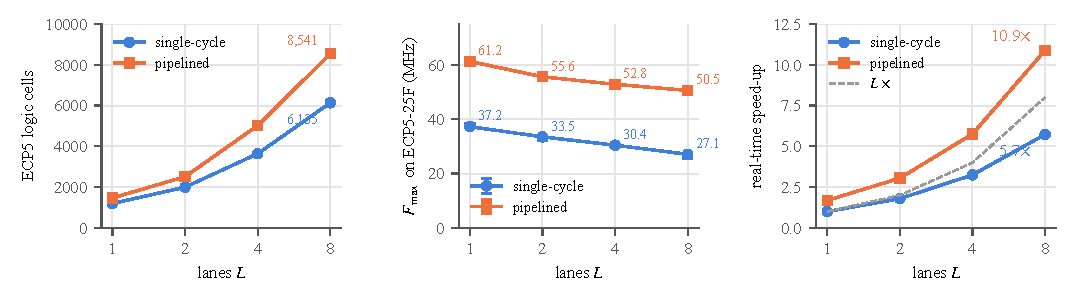
\includegraphics[width=\textwidth]{figures/p2_fpga.pdf}
\caption{Both cores on the ECP5-25F against lane count: logic cells after place and
route; $F_{\max}$, median of three placement seeds with the range; and real-time speed-up
over the single-cycle one-lane core, the mean over eight workloads of $N = 256$
elements (dashed: $L\times$).}
\label{fig:fpga2}
\end{figure*}

In the single-cycle core the frequency falls from 37.3~MHz at one lane to 27.1~MHz at
eight, 27\% lower; the spread between placement seeds is at most 1.7~MHz.
Because every instruction executes in one cycle, the critical path crosses the whole
datapath, from the instruction block RAM through the register reads, a lane ALU, the
result selection and, for reductions, the adder tree to the scalar register write.

The pipeline raises $F_{\max}$ by $1.64\x$ at one lane and $1.87\x$ at eight, and the
clock falls more slowly with the lane count: by 17\% from one to eight lanes, against
27\%, because the adder tree, which deepens with $L$, now has a stage of its own. The
slowest path moves from a whole instruction to a single stage: at one lane the fetch
loop, in which the decoded branch guess selects the next fetch address; from two lanes
on the execute stage, from a forwarded operand through the lane multiplier into the X/W
register, a path that widens with $L$ because the forwarding multiplexers are $16L$ bits
wide.

The price is logic: 39\% more ECP5 cells at eight lanes and 291 more flip-flops for the
pipeline registers. On Artix-7, whose six-input LUTs absorb the wide multiplexers
better, the increase is 7\% (3,600 against 3,372 LUTs, 17.3\% and 16.2\% of the device),
and both cores use eight DSP slices, one per lane. As noted in Section~\ref{sec:why}, the new instructions also cost the single-cycle core
logic and clock.

\subsection{Cycle Breakdown}
Fig.~\ref{fig:cyc2}(a) splits the cycles at eight lanes into instructions and extra
cycles. The two cores need almost the same number of cycles, the pipelined core 0.4\%
fewer on average, for different reasons. The single-cycle core pays one extra cycle per
load. The pipelined core pays nothing for loads but one cycle whenever a loaded
register, a reduction sum or a masked result is used by the very next instruction,
plus two fixed cycles. A pass therefore takes $b + \ell$ cycles on the single-cycle core
and $b + \sigma$ on the pipelined core (Table~\ref{tab:cyc2}). \texttt{saxpy} has no
stalls at all and \texttt{vadd} one stall for two loads, so the pipelined core needs 62
and 30 fewer cycles. On \texttt{relu}, \texttt{threshold}, \texttt{dot} and
\texttt{brighten} the stalls cancel the saved load cycles and the pipelined core needs two
more cycles, its fixed cost. On \texttt{abs} and \texttt{sumpos}, with two stalls but one
load per pass, it needs 34 more.

\begin{figure*}[t]
\centering
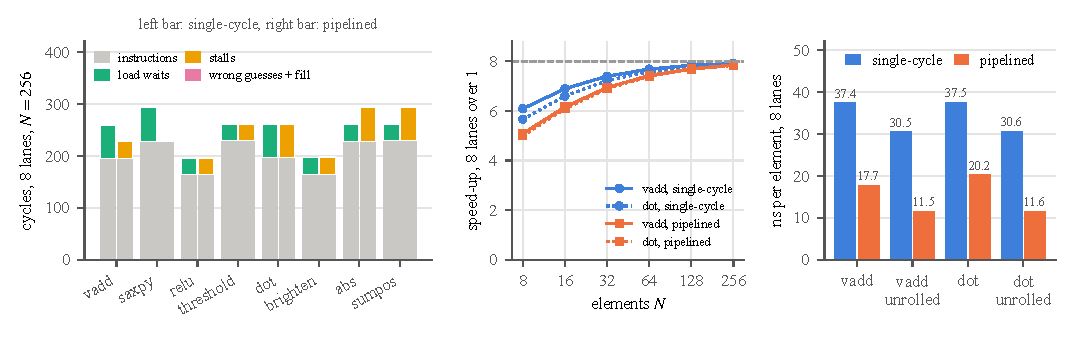
\includegraphics[width=\textwidth]{figures/p2_cycles.pdf}
\caption{(a) Cycles at eight lanes split into instructions and extra cycles (left bar of
each pair: single-cycle core; right: pipelined). (b) Cycle speed-up of eight lanes over
one against the problem size $N$, measured on the RTL. (c) Time per element at eight
lanes for the original loops and loops unrolled four times.}
\label{fig:cyc2}
\end{figure*}

\subsection{Real-Time Speed-Up}
Because the cycle counts are so close, the pipeline's advantage is its clock. In real
time the eight-lane pipelined core is $1.90\x$ faster than the eight-lane single-cycle
core, from $1.65\x$ on \texttt{abs} and \texttt{sumpos} (two stalls but one load per pass) to
$2.37\x$ on \texttt{saxpy} (Table~\ref{tab:cyc2}); at one lane the ratio is $1.68\x$ and it grows
with $L$ because the pipelined clock falls more slowly. Against the scalar baseline, the
single-cycle one-lane core, the eight-lane single-cycle core is $5.73\x$ faster and the
eight-lane pipelined core $10.88\x$ (Table~\ref{tab:scale} and
Fig.~\ref{fig:fpga2}, right). The pipelined core alone, at one lane, is $1.68\x$ faster
than the scalar baseline: pipelining and SIMD contribute separately, and their product
exceeds the lane count.

\subsection{Throughput and Area Efficiency}
Dividing the elements processed by the real time gives throughput, and dividing that by
the logic used gives area efficiency (Table~\ref{tab:eff}). At eight lanes the pipelined
core processes 53.8 million elements per second against 28.5 for the single-cycle core,
and 6.30 against 4.64 per thousand logic cells: the extra pipeline logic more than pays
for itself, so the pipelined core is the more efficient design at every lane count, not
only the faster one. For both cores efficiency is roughly flat with $L$, because the
lanes add logic and throughput almost in proportion while the shared control is a small
part of the total.

\begin{table}[t]
\centering
\caption{Throughput and Area Efficiency (Mean of Eight Workloads)}
\label{tab:eff}
\footnotesize
\begin{tabular}{@{}rrrrr@{}}
\toprule
 & \multicolumn{2}{c}{M elements/s} & \multicolumn{2}{c}{per 1,000 cells} \\
\cmidrule(lr){2-3}\cmidrule(lr){4-5}
$L$ & single & pipe & single & pipe \\
\midrule
1 & 5.0  & 8.3  & 4.15 & 5.67 \\
2 & 8.9  & 15.1 & 4.47 & 6.00 \\
4 & 16.1 & 28.5 & 4.43 & 5.67 \\
8 & 28.5 & 53.8 & 4.64 & 6.30 \\
\bottomrule
\end{tabular}
\end{table}

\subsection{Problem Size}
Fig.~\ref{fig:cyc2}(b) shows the cycle speed-up of eight lanes over one for $N = 8$ to
256, measured on the RTL for \texttt{vadd} and \texttt{dot} on both cores
(Table~\ref{tab:size}). At $N = 8$ the eight-lane loop runs once, the set-up code is a
large share of the work and the speed-up is $5.0$--$6.1\x$; by $N = 256$ it is within 2\%
of the ideal $8\x$. This is Amdahl's law with a serial fraction that shrinks as $N$
grows, as Gustafson~\cite{gustafson} observed for scaled problems. The pipelined core
falls slightly further at small $N$ because its fixed part, which includes the pipeline
fill and the final wrong guess, is larger. For \texttt{vadd} on the single-cycle core the
model~\eqref{eq:model} predicts $7.99\x$ at $N = 4096$; that size was not run, because
more than 341 elements do not fit the one-lane build's data memory.

\begin{table}[t]
\centering
\caption{Cycle Speed-Up of 8 Lanes Over 1 Against Problem Size}
\label{tab:size}
\footnotesize
\begin{tabular}{@{}rrrrr@{}}
\toprule
 & \multicolumn{2}{c}{\texttt{vadd}} & \multicolumn{2}{c}{\texttt{dot}} \\
\cmidrule(lr){2-3}\cmidrule(lr){4-5}
$N$ & single & pipe & single & pipe \\
\midrule
8   & 6.09 & 5.08 & 5.67 & 5.00 \\
16  & 6.89 & 6.16 & 6.60 & 6.09 \\
32  & 7.40 & 6.94 & 7.22 & 6.89 \\
64  & 7.69 & 7.43 & 7.59 & 7.40 \\
128 & 7.84 & 7.70 & 7.79 & 7.69 \\
256 & 7.92 & 7.85 & 7.89 & 7.84 \\
\bottomrule
\end{tabular}
\end{table}

\subsection{Unrolling and Instruction Order}
In one pass of \texttt{vadd} at eight lanes on the single-cycle core only one of the
eight cycles does arithmetic; two loads take four cycles, and the store and the loop
control take three (Fig.~\ref{fig:timing}). The ALUs are idle most of the time, and the
limit is issue, not memory bandwidth: one instruction per cycle, loads that are not
overlapped, and the loop control. Unrolling \texttt{vadd} and \texttt{dot} four times,
with all eight loads placed first, attacks both. Both cores execute about 25\% fewer
instructions (195 to 147 and 196 to 148), because the loop overhead is paid once per four
vectors. Only the pipelined core also loses its stalls: every register is loaded several
instructions before it is used, and in \texttt{dot\_unroll} each \texttt{VDOT} writes its
own register, consumed four instructions later. The pipelined core then completes one
instruction per cycle (147 instructions in 149 cycles for \texttt{vadd\_unroll}), and the
time per element falls from 17.7 to 11.5~ns for \texttt{vadd} and from 20.2 to 11.6~ns
for \texttt{dot} (Fig.~\ref{fig:cyc2}(c)). The single-cycle core gains only the
instruction count (259 to 211 and 260 to 212 cycles, 37.4 to 30.5~ns and 37.5 to
30.6~ns per element), because its loads cost an extra cycle wherever they are. The
unrolled programs on the eight-lane pipelined core are $18.6\x$ faster than the original
programs on the scalar single-cycle core (mean of $18.7\x$ and $18.6\x$ for \texttt{vadd}
and \texttt{dot}), and $15.1\x$ faster than the same unrolled programs on it. The
hardware sets the clock; the order of the instructions decides how many clocks are
wasted.

\subsection{Limitations and Threats to Validity}
\begin{itemize}
\item $F_{\max}$ is nextpnr's static-timing estimate without pin constraints, for one
      device and speed grade. The Artix-7 figures are Yosys estimates without timing;
      the Vivado flow for the Basys-3 board, which would give exact Artix-7 timing, could
      not be run because Vivado does not support the development machine. The board
      check simulates the FPGA top; the design has not run on a physical board.
\item Real time assumes a memory that delivers a 128-bit word per cycle, as the on-chip
      block RAM does. No power or energy was measured, and the kernels are short and
      regular.
\item The branch predictor is static, which suits these loops but would mispredict
      data-dependent branches.
\item Elements are 16-bit integers only, and there is one mask register. \texttt{VDOT}
      keeps only the low 16 bits of each product, so its inputs must be small enough for
      the products to fit; a widening multiply would remove this limit.
\item A program must be reassembled for each lane count, because the loop count $N/L$ is
      a constant; there is no \texttt{vsetvli}-style length instruction.
\end{itemize}

% =============================================================================
\section{Conclusion}\label{sec:conclusion}
A lane-parameterised SIMD unit with a one-lane scalar baseline, implemented as a
single-cycle core and as a four-stage pipelined core with the same 55-instruction set,
gives a clean answer to the project's questions. In clock cycles both cores scale almost
perfectly with the lanes: eight lanes need $7.89\x$ (single-cycle) and $7.83\x$
(pipelined) fewer cycles than one. The single-cycle core pays for its width in clock
rate, falling from 37.3 to 27.1~MHz, so its real-time speed-up at eight lanes is $5.73\x$.
Measuring its critical path located the limit in three nearly equal pieces, and a
four-stage pipeline built around them raised the eight-lane clock to 50.6~MHz.
Forwarding, write-through register files, three one-cycle stall rules and
backward-taken branch prediction keep the cycle count within 0.4\% of the single-cycle
core, so the clock gain becomes a $1.90\x$ real-time gain at equal lane count, and the
eight-lane pipelined core is $10.88\x$ faster than the scalar single-cycle design
($18.6\x$ with unrolled loops), for 39\% more logic and with better area efficiency.
Masked execution and saturating arithmetic bring the instruction set closer to
production SIMD extensions without a new register-file read port. A golden model that
predicts the cycle count of both cores made the pipeline verifiable to the same standard
as the single-cycle design: every workload, directed test, mid-run reset and random
program agrees with it, and every injected and planted bug is caught. The remaining
gains lie in software (instruction scheduling and unrolling) and in running the design
on a board, with measured power per operation.

% =============================================================================
\section*{Code and Data Availability}
All RTL, testbenches, programs, scripts, results and figures are in the repository
named on the first page. \texttt{make test} runs the lint, unit testbenches, software
tests, both cores' system, directed, reset and random-program runs and the board checks;
\texttt{make fuzz} runs 8,000 random programs; \texttt{make perf}, \texttt{make sweep}
and \texttt{make syn} regenerate the cycle counts, the size sweep and the FPGA results;
and \texttt{make report} rebuilds the figures and the papers from them.

\section*{Individual Contributions}
\textbf{Mahir Abdullah} (lead): the architecture, instruction format and block interfaces
that the team built against; the vector control unit with early instruction fetch and
two-cycle load; core integration with performance counters; the critical-path analysis
and the pipeline design, with the shared decoder, the pipelined core and the hazard unit;
masked execution across both cores; the instruction-level golden model with its cycle
model for both cores, the workload runner and the system testbench; the directed, hazard,
mask, long-branch and mid-run reset tests, the random-program fuzzer for both cores and
the planted-bug campaign; the repository, continuous integration and documentation; and
this paper.

\textbf{Krishiv Gupta}: the lane ALU with its \texttt{generate}-based array, including
signed and unsigned compares and arithmetic shifts and the saturating \texttt{ADDS} and
\texttt{SUBS} with hand-checked saturation cases and clamp coverage, and its 257,689-check
testbench, which also confirms that no carry crosses a lane; the FPGA top with block-RAM
memories and power-on reset that builds either core; the board checks of both cores; and
the ECP5 and Artix-7 synthesis sweep of both cores, with the Vivado script, the Basys-3
constraints and the resource, $F_{\max}$ and slowest-path analysis.

\textbf{Abhiman Singh}: the vector and scalar register files, with two read ports and
one write port each, a hard-wired zero register and the debug port that forms the scalar
interface, and later the per-lane write enables, the lane mask register and the
write-through option; and their testbench, which builds each file in both modes and
checks it against a shadow model, covering read-during-write behaviour and random
cycles.

\textbf{Gogulamudi Jayadeep}: the lane multiplexers and the result combiner with its
$\log_2 L$ adder tree, and later its masked lane sums and lane flags, verified at every
lane count; and the speed-up analysis: cycle counts for 1, 2, 4 and 8 lanes for both
cores, the real-time comparison, the cycle breakdown, the problem-size sweep, the unrolled
programs, elements per cycle and the figures.

\textbf{Ashish Kushwaha}: the two-pass assembler with labels, constants and
line-numbered error messages, later extended for the saturating, masked and
\texttt{VMSK} instructions, with its tests; and the workload programs, including the
branch-free threshold kernel, the \texttt{brighten}, \texttt{abs} and \texttt{sumpos}
programs, and the instruction-coverage program with full coverage of the new
instructions.

\section*{Acknowledgment}
The authors thank the developers of Icarus Verilog, Verilator, Yosys and nextpnr, whose
open tools make every result in this paper reproducible.
